\documentclass[border=5mm]{standalone}
\usepackage{tikz}

\begin{document}
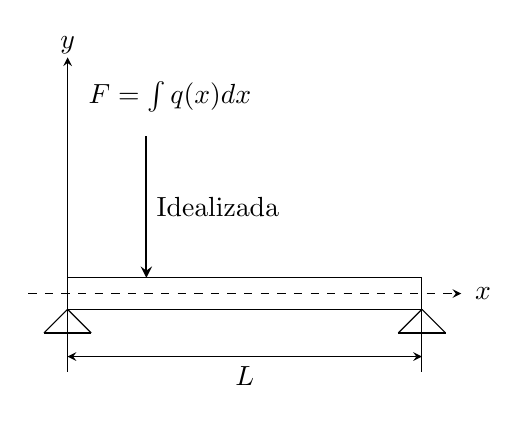
\begin{tikzpicture}
	\draw [-stealth, dashed] (-0.5, 0) -- (5, 0) node [near end, pos=1.05] {$x$};
	\draw [-stealth] (0, 0) -- (0, 3) node [near end, pos=1.05] {$y$};
	\draw (0, -0.2) rectangle (4.5, 0.2);

	\draw (0, -0.2) -- (-0.3, -0.5);
	\draw (0, -0.2) -- (0.3, -0.5);
	\draw (-0.3, -0.5) -- (0.3, -0.5);

	\draw (4.5, -0.2) -- (4.2, -0.5);
	\draw (4.5, -0.2) -- (4.8, -0.5);
	\draw (4.2, -0.5) -- (4.8, -0.5);

	\draw (0, 0) -- (0, -1);
	\draw (4.5, 0) -- (4.5, -1);

	\draw [>=stealth, <->] (0, -0.8) -- (4.5, -0.8) node [midway, below] {$L$};

	\draw [-stealth, thick] (1, 2) -- (1, 0.2) node [right, midway] {Idealizada};

	\node at (1.3, 2.5) {$F = \int q (x) dx$};

\end{tikzpicture}
\end{document}